\section{Systems}
\label{sec:systems}

All systems receive one sentence and return a possibly empty list of categories (empty means fair), in the same file format, so that one evaluation code scores them all.

\subsection{Baselines}
\label{sec:baselines}

\begin{itemize}
  \item \textbf{Always fair} never flags anything: the floor that shows why micro-F1 alone is misleading.
  \item \textbf{TF-IDF + SVM:} word 1--3-grams, a linear SVM per category, with the regularisation $C=10$ chosen on validation.
  \item \textbf{Plain LLM:} \texttt{gpt-4.1-mini-2025-04-14}~\citep{openai2025gpt41}, zero-shot. The system prompt contains the task, based on Article 3(1) of the Directive, the eight category cards and a few rules. For example, a sentence that only mentions a topic is not unfair, and a clearly fair clause is not unfair. The model answers with a strict JSON schema: an explanation first, then a yes/no verdict and the categories (``reason, then decide''). Temperature 0, a fixed seed and a dated model snapshot make the runs as reproducible as the API allows.
  \item \textbf{Legal-BERT}~\citep{chalkidis2020legalbert} (\texttt{nlpaueb/legal-bert-base-uncased}), fine-tuned for multi-label classification: learning rate $3\cdot10^{-5}$, batch size 16, sequences of up to 256 tokens, early stopping on validation macro-F1 with patience 3. We train three seeds and report the mean and standard deviation; each seed takes 7--11 minutes on a laptop GPU (RTX 4050, 6\,GB).
\end{itemize}

\subsection{Retrieval}
\label{sec:retrieval}

The retriever embeds the sentence and the documents of the knowledge base with BAAI/bge-m3~\citep{chen2024bgem3}, a multilingual model, so that the same English index also serves German, Italian and Polish sentences. For a knowledge base of 5,584 documents, exact cosine search with numpy is fast enough and needs no vector database. For each sentence the retriever returns:
\begin{itemize}
  \item the 8 most similar training sentences, with their expert labels, fair or unfair;
  \item the 5 most similar legal rationales;
  \item the provisions those rationales rely on, at most 6.
\end{itemize}

Table~\ref{tab:retrieval} measures retrieval on the validation set. With 8 examples and 5 rationales, 97\% of the unfair sentences receive at least one example and one rationale of their own category, so the evidence the model needs is almost always in its context. For fair sentences, 93\% of the retrieved examples are fair, which is evidence against false alarms.

\begin{table}[ht]
\centering\small
\caption{Retrieval quality on validation (230 unfair, 2,045 fair sentences). Hit@$k$: share of unfair sentences with at least one retrieved item of their category. Purity@$k$: share of fair examples among those retrieved for fair sentences.}
\label{tab:retrieval}
\begin{tabular}{@{}rrrr@{}}
\toprule
$k$ & Example hit@$k$ & Rationale hit@$k$ & Fair purity@$k$ \\
\midrule
1 & 72.6 & 78.7 & 95.9 \\
3 & 90.9 & 94.3 & 94.2 \\
5 & 94.8 & 96.5 & 93.7 \\
8 & 97.4 & 97.8 & 92.7 \\
\bottomrule
\end{tabular}
\end{table}

The retrieved examples alone already carry a strong signal. A \textbf{kNN vote} flags a category when at least $t$ of the $k$ most similar training sentences have it. It needs no training and no language model; on validation the best setting is $k=3$, $t=2$.

\subsection{The RAG system}
\label{sec:rag}

The RAG system uses the same model, settings, task description and category cards as the plain LLM, so that the only difference is the retrieved knowledge (Figure~\ref{fig:pipeline}). The system prompt adds a short section on how to use the evidence: judge the sentence itself, since a similar item can have a different meaning, and remember that similar sentences labelled fair are evidence of fairness. The user message lists the retrieved examples with their labels, the rationales and the provisions, each with its id in brackets, followed by the sentence. The answer schema adds a field \texttt{cited\_ids}, between the explanation and the verdict, for the items the decision relies on. After the answer, a \textbf{citation check} compares the cited ids with those actually retrieved, so that an invented source is detected and ignored. The system prompt is identical for every sentence, which lets the API reuse it from its prompt cache.

\begin{figure}[ht]
\centering
\begin{tikzpicture}[
  box/.style={draw=black!55, rounded corners=2pt, align=center, font=\small, inner sep=4pt, minimum height=9mm},
  kb/.style={box, fill=black!4},
  arr/.style={-{Stealth[length=2mm]}, black!65}]
\node[box, text width=2.2cm] (s) at (0,0) {Sentence of a Terms of Service};
\node[box, text width=1.5cm] (r) at (2.75,0) {Retrieval (bge-m3)};
\node[kb, text width=3.7cm] (k) at (6.25,1.05) {8 expert-labelled examples\\5 legal rationales\\$\le$6 legal provisions};
\node[box, text width=3.7cm] (v) at (6.25,-1.05) {Precedent votes: how many of the 8 examples have each category};
\node[box, text width=2.7cm] (l) at (10.25,1.05) {LLM: explanation, cited ids, verdict, categories};
\node[box, text width=1.8cm] (c) at (13.45,1.05) {Citation check};
\node[box, text width=2.0cm] (g) at (13.45,-1.05) {Evidence gate\\($\ge$3 of 8)};
\node[kb] (o) at (10.0,-2.75) {Verdict, explanation\\and evidence for the user};
\draw[arr] (s) -- (r);
\draw[arr] (r.north) |- (k.west);
\draw[arr] (r.south) |- (v.west);
\draw[arr] (k) -- (l);
\draw[arr] (l) -- (c);
\draw[arr] (c) -- (g);
\draw[arr] (v) -- (g);
\draw[arr] (g.south) |- (o.east);
\end{tikzpicture}
\caption{The RAG system with the evidence gate. The language model sees the retrieved knowledge; the gate sees only the expert labels of the most similar training sentences.}
\label{fig:pipeline}
\end{figure}

\subsection{The evidence gate}
\label{sec:gate}

On validation, retrieval helped the language model but did not stop it from flagging sentences because of their topic. Of the 210 fair sentences the RAG system flagged, 132 had at least 6 of their 8 most similar training sentences labelled fair by the experts, and 44 had all 8. The \textbf{evidence gate} turns this observation into a transparent rule: a category proposed by the model is kept only if at least $m$ of the $k$ most similar expert-labelled training sentences have it. A flagged clause then has both a legal explanation and expert precedents.

The values of $k$ and $m$ were chosen on the validation set by a rule fixed in advance: the best macro-F1 among the settings with a recall of unfair sentences of at least 80\%, because for consumer protection a missed unfair clause is worse than a false alarm. If no setting reached 80\%, the rule would take the highest recall. The rule selects $k=8$, $m=3$ (Figure~\ref{fig:gate}). On validation, the gate removes the flags of 171 sentences: 149 false alarms, but also 22 unfair clauses, so recall drops from 92.2\% to 82.6\%. Section~\ref{sec:ethics-consequences} discusses this trade-off.

\begin{figure}[ht]
\centering
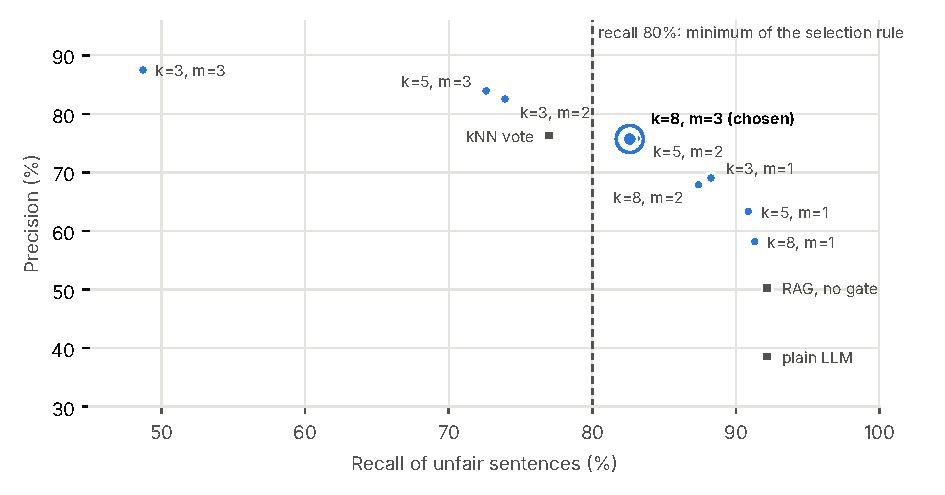
\includegraphics[width=0.8\textwidth]{gate_tradeoff.pdf}
\caption{Precision and recall of unfair sentences on validation for the nine settings of the evidence gate (blue), and for three systems without it (grey). The selection rule takes the best macro-F1 to the right of the dashed line.}
\label{fig:gate}
\end{figure}

\subsection{Open-weight replication}
\label{sec:openweight}

The multilingual evaluation needed about 10,000 sentences per system, more than our API budget allowed. We therefore replicated the whole pipeline with an open-weight model, Qwen3.6-27B in FP8~\citep{qwen2026}, served with vLLM~\citep{kwon2023vllm} on one NVIDIA L40 (48\,GB) of the DISI cluster of the University of Bologna. The setup keeps the same prompts, answer schema, knowledge base, gate rule and evaluation, and switches off the model's ``thinking'' mode so that it answers directly, like gpt-4.1-mini. The replication serves two purposes: all comparisons across languages use one model, and it tests whether our findings depend on a particular commercial model. It also keeps the data on infrastructure the university controls, which Section~\ref{sec:ethics-gdpr} discusses.

\subsection{Implementation}

The code is a Python package (\texttt{src/claudette\_rag}) with command-line scripts and 54 unit tests. Every answer of a language model is appended to a log as soon as it arrives, so an interrupted run resumes without paying twice. The predictions, explanations with their retrieved and cited ids, and evaluation reports of every run are saved in the repository. Choices were made on the validation set, and the test set was used once per system. The main system (full RAG with the gate) was declared before its test run.
